\documentclass[10pt,a4paper]{article}
\usepackage[margin=2.2cm]{geometry}
\usepackage{amsmath,amssymb,bm}
\usepackage{graphicx}
\usepackage{booktabs}
\usepackage{array}
\usepackage{xcolor}
\usepackage{caption}
% clickable references: every Fig./Table/Eq./Sec. number jumps to its target
\usepackage{hyperref}
\hypersetup{colorlinks=true,linkcolor=blue!55!black,urlcolor=blue!55!black,
            citecolor=blue!55!black}
\captionsetup{font=small,labelfont=bf}
\setlength{\parskip}{0.45em}
\setlength{\parindent}{0pt}

% every number below is written by make_note.py from one stored device
\newcommand{\devname}{sample\_10}
\newcommand{\res}{100}
\newcommand{\vxlo}{-1.280}
\newcommand{\vxhi}{0.720}
\newcommand{\vylo}{-1.108}
\newcommand{\vyhi}{0.892}
\newcommand{\gam}{0.01}
\newcommand{\temp}{10^{-5}}
\newcommand{\npeak}{5}
\newcommand{\Cddnm}{\begin{pmatrix}1.3571 & 0.5329 \\ 0.5329 & 0.4363\end{pmatrix}}
\newcommand{\Cgdnm}{\begin{pmatrix}1.8950 & 0.4904 & 0.0943 \\ 0.0625 & 3.0132 & 0.0191\end{pmatrix}}
\newcommand{\Cdsnm}{\begin{pmatrix}0.0538 & 0.0487\end{pmatrix}}
\newcommand{\Cgsnm}{\begin{pmatrix}0.0718 & 0.0480 & 0.2623\end{pmatrix}}
\newcommand{\Cmax}{\begin{pmatrix}4.3697 & -0.5329 \\ -0.5329 & 4.0640\end{pmatrix}}
\newcommand{\Cinv}{\begin{pmatrix}0.2326 & 0.0305 \\ 0.0305 & 0.2501\end{pmatrix}}
\newcommand{\Amat}{\begin{pmatrix}0.4426 & 0.2059 & 0.0225 \\ 0.0734 & 0.7684 & 0.0077\end{pmatrix}}
\newcommand{\Cfull}{\begin{pmatrix}4.4235 & -0.5329 & -0.0538 \\ -0.5329 & 4.1127 & -0.0487 \\ -0.0538 & -0.0487 & 0.4846\end{pmatrix}}
\newcommand{\ConeOne}{4.3697}
\newcommand{\dOneOne}{1.3571}
\newcommand{\dOneTwo}{0.5329}
\newcommand{\gOneSum}{2.4797}
\newcommand{\sSens}{0.4846}
\newcommand{\CssFull}{0.4846}
\newcommand{\pixV}{(-0.2703,\ -0.0981,\ 0)}
\newcommand{\pixNg}{(0.5603,\ 0.3126)}
\newcommand{\pixN}{(1,\ 0)}
\newcommand{\Ftable}{$n_1=0$ & $0.1081$ & $0.1677$ & $0.7274$ & $1.7872$ \\
$n_1=1$ & $\mathbf{0.0610}$ & $0.1815$ & $0.8022$ & $1.9230$ \\
$n_1=2$ & $0.4790$ & $0.6605$ & $1.3422$ & $2.5240$ \\
$n_1=3$ & $1.3621$ & $1.6047$ & $2.3473$ & $3.5901$ \\}
\newcommand{\slopeOne}{-2.149}
\newcommand{\slopeTwo}{-0.096}
\newcommand{\slopeInter}{0.656}
\newcommand{\mslopeOne}{-2.148}
\newcommand{\nOne}{76}
\newcommand{\pairOne}{(0,0)}
\newcommand{\pairTwo}{(0,0)}
\newcommand{\pairInter}{(1,3)}
\newcommand{\mslopeTwo}{-0.097}
\newcommand{\nTwo}{50}
\newcommand{\mslopeInter}{1.000}
\newcommand{\nInter}{4}
\newcommand{\dVone}{0.5254}
\newcommand{\dVtwo}{0.3254}
\newcommand{\EcOne}{0.2326}
\newcommand{\EcTwo}{0.2501}
\newcommand{\Em}{0.0305}
\newcommand{\linefrac}{5.3}
\newcommand{\nstates}{16}
\newcommand{\statelist}{(0,0), (0,1), (0,2), (0,3), (1,0), (1,1), (1,2), (1,3), (2,0), (2,1), (2,2), (2,3), (3,0), (3,1), (3,2), (3,3)}
\newcommand{\zmaxdiff}{exactly zero}
\newcommand{\zlo}{5.53}
\newcommand{\zhi}{7.18}
\newcommand{\detmin}{1.421}
\newcommand{\detminovergam}{142}
\newcommand{\npix}{10000}
\newcommand{\checktable}{C matches QArray & \textbf{pass} \\
C\_full matches QArray & \textbf{pass} \\
hole sign: cgd = -C\_g & \textbf{pass} \\
ground state = QArray DotArray (all pixels) & \textbf{pass} \\
ground state = stored charge\_states.npy & \textbf{pass} \\
label = stored ground truth (interior) & \textbf{pass} \\
sensor signal = QArray (all pixels) & \textbf{pass} \\
QArray V grid = ours (V3 = 0) & \textbf{pass} \\}


\newcommand{\n}{\mathbf{n}}
\newcommand{\V}{\mathbf{V}}
\newcommand{\nG}{\mathbf{n}_g}
\newcommand{\Cg}{C_g}
\newcommand{\code}[1]{\texttt{\detokenize{#1}}}

\title{From gate voltages to transition lines:\\
how the simulator behind the dataset works}
\author{Notes for \emph{probabilistic-csd-reconstruction}}
\date{26 September 2026}

\begin{document}
\maketitle

\begin{abstract}
\noindent
Every device in the dataset is simulated with QArray~1.6.0 in the
constant-capacitance model. This note follows one device from its 14
sampled capacitances to the two arrays the study uses: the charge-sensor
map the rays are measured on, and the binary transition-line map the
network is trained against. Each step is written as an equation and then
re-implemented independently in \code{make_note.py}, which compares the
result with what QArray and this repository actually produced for the
stored device \devname. All eight comparisons agree exactly
(Table~\ref{tab:checks}), so the equations below are the ones the code
evaluates, not a textbook paraphrase of them. All numbers are for
\devname.
\end{abstract}

% ---------------------------------------------------------------------------
\section{The ingredients: 14 capacitances}

A device is two quantum dots (1, 2), one sensor dot (s) and three gates
(g1, g2, g3). QArray takes four \emph{non-Maxwell} matrices, whose
entries are the individual capacitors of the circuit
(Fig.~2(a) of the paper). For \devname\ they are
\begin{equation}
C_{dd}^{\rm nm} = \Cddnm,\quad
C_{gd}^{\rm nm} = \Cgdnm,
\label{eq:nm}
\end{equation}
\begin{equation*}
C_{ds}^{\rm nm} = \Cdsnm,\qquad
C_{gs}^{\rm nm} = \Cgsnm .
\end{equation*}
The diagonal of $C_{dd}^{\rm nm}$ holds each dot's capacitance to ground
(QArray's ``self'' capacitance, $d_1d_1=\dOneOne$); the off-diagonal
entry is the interdot capacitor ($d_1d_2=\dOneTwo$). Rows of $C_{gd}^{\rm
nm}$ are dots and columns are gates. That is
$3 + 6 + 2 + 3 = 14$ numbers. \textbf{There is no capacitance from the
sensor to ground}: QArray has no argument for one, and the code passes
none (Sec.~\ref{sec:sensor}).

% ---------------------------------------------------------------------------
\section{Step 1 --- the capacitance matrix}

QArray's \code{convert_to_maxwell} turns the circuit into the
total-capacitance (Maxwell) matrix $C$:
\begin{equation}
C_{ii} = \sum_j \big(C_{dd}^{\rm nm}\big)_{ij} + \sum_g
\big(C_{gd}^{\rm nm}\big)_{ig},
\qquad
C_{ij} = -\big(C_{dd}^{\rm nm}\big)_{ij}\quad (i\neq j).
\label{eq:maxwell}
\end{equation}
The diagonal is the \emph{total} capacitance of a dot: everything
attached to it. The off-diagonal is minus the interdot coupling.

\paragraph{Example.} For dot~1,
$C_{11} = \dOneOne + \dOneTwo + \gOneSum = \ConeOne$, where
$\gOneSum$ is the sum of its three gate capacitors. In full,
\begin{equation}
C = \Cmax,\qquad
C^{-1} = \Cinv .
\end{equation}
$C^{-1}_{11}=\EcOne$ and $C^{-1}_{22}=\EcTwo$ set the charging energy of
each dot; $C^{-1}_{12}=\Em$ is the electrostatic coupling between them.
The gate matrix used from here on is $\Cg \equiv C_{gd}^{\rm nm}$
(2$\times$3).

% ---------------------------------------------------------------------------
\section{Step 2 --- the energy of a charge configuration}

Let $\n=(n_1,n_2)$ be the number of carriers on each dot and
$\V=(V_1,V_2,V_3)$ the gate voltages. QArray's \code{free_energy}
evaluates
\begin{equation}
\boxed{\;F(\n;\V) = (\n-\nG)^{\mathsf T}\, C^{-1}\, (\n-\nG),
\qquad \nG = -\,\Cg\,\V \;}
\label{eq:F}
\end{equation}
This is the electrostatic energy of the constant-capacitance model divided
by $e^2/2$; QArray works in dimensionless units throughout.

Three things are worth knowing about Eq.~\eqref{eq:F}.
\begin{itemize}
\item $\nG$ is the charge the gates \emph{induce} on each dot. It is
continuous in $\V$; $\n$ is an integer vector. The energy is lowest when
$\n$ is as close as possible to $\nG$, measured with the metric $C^{-1}$.
\item \textbf{The minus sign is the carrier.} Both QArray models are built
with holes (\code{charge_carrier="hole"}, the default of
\code{ChargeSensedDotArray} as well), and for holes QArray stores
$-|C_{gd}|$. So $\nG$ grows as the gate voltage becomes \emph{more
negative}: in every stability diagram of this study the occupation
increases towards the lower left.
\item Only $V_1$ and $V_2$ are swept. $V_3$ is held at 0; the check
``QArray V grid = ours'' in Table~\ref{tab:checks} confirms it.
\end{itemize}

% ---------------------------------------------------------------------------
\begin{figure}[t]
\centering
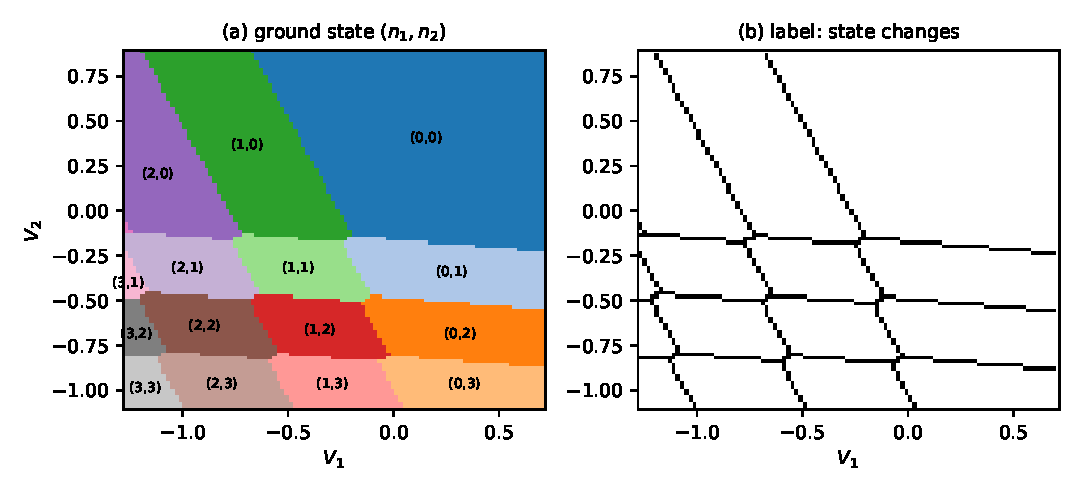
\includegraphics[width=0.92\linewidth]{figures/states_and_label.pdf}
\caption{(a) Ground state $\n^*(\V)$, Eq.~\eqref{eq:gs}. (b) The label,
Eq.~\eqref{eq:label}: every boundary in (a), one pixel wide.}
\label{fig:states}
\end{figure}

\section{Step 3 --- the ground state}

At every point of the window the dots are open to a reservoir, so the
occupation is whatever minimises the energy:
\begin{equation}
\n^{*}(\V) = \arg\min_{\n\in\mathbb{N}_0^2} F(\n;\V).
\label{eq:gs}
\end{equation}
The simulation temperature is $T=\temp$ (in QArray's units), so this is
the zero-temperature ground state. \code{make_note.py} evaluates
Eq.~\eqref{eq:gs} by brute force over $n_i=0,\dots,5$ and obtains the same
occupation as QArray at all \npix\ pixels.

\paragraph{Worked example.} At the centre pixel,
$\V=\pixV$, which gives $\nG=\pixNg$. Table~\ref{tab:F} lists $F$ for
the 16 lowest configurations. The minimum (bold) is $\n^*=\pixN$: dot~1
has 0.56 induced charges and rounds up, dot~2 has 0.31 and rounds down,
and the coupling term does not change the outcome here.

\begin{table}[h]
\centering
\caption{$F(\n;\V)$ at the centre pixel, $\nG=\pixNg$.}
\label{tab:F}
\begin{tabular}{l cccc}
\toprule
 & $n_2=0$ & $n_2=1$ & $n_2=2$ & $n_2=3$\\
\midrule
\Ftable
\bottomrule
\end{tabular}
\end{table}

Across the whole window of \devname\ the ground state takes
\nstates\ values, \statelist\ (Fig.~\ref{fig:states}(a)).

% ---------------------------------------------------------------------------
\section{Step 4 --- where the transition lines are}

A transition line is where the ground state changes, i.e.\ where two
configurations $\n$ and $\n+\mathbf{d}$ have the same energy. From
Eq.~\eqref{eq:F},
\begin{equation}
F(\n+\mathbf{d};\V)-F(\n;\V)
= \mathbf{d}^{\mathsf T}C^{-1}\mathbf{d}
+ 2\,\mathbf{d}^{\mathsf T}C^{-1}\n
+ 2\,\mathbf{d}^{\mathsf T}A\,\V = 0,
\qquad A \equiv C^{-1}\Cg .
\label{eq:degen}
\end{equation}
The condition is \emph{linear} in $\V$, so every boundary is a straight
segment. Three kinds of step $\mathbf{d}$ occur:
\begin{center}
\begin{tabular}{lll}
\toprule
$\mathbf{d}$ & transition & what happens \\
\midrule
$(1,0)$ & dot-1 line & one carrier enters dot 1 from the reservoir\\
$(0,1)$ & dot-2 line & one carrier enters dot 2\\
$(1,-1)$ & interdot line & one carrier moves from dot 2 to dot 1\\
\bottomrule
\end{tabular}
\end{center}
With $V_3=0$, Eq.~\eqref{eq:degen} gives the slope of each family in the
$(V_1,V_2)$ plane:
\begin{equation}
\frac{dV_2}{dV_1} = -\,\frac{(\mathbf{d}^{\mathsf T}A)_1}
{(\mathbf{d}^{\mathsf T}A)_2},
\qquad
A = \Amat .
\label{eq:slope}
\end{equation}
$A$ is the lever-arm matrix: $A_{ig}$ is how strongly gate $g$ moves the
energy of dot $i$. The first two columns are what shape the diagram.

\paragraph{Example: slopes.} Eq.~\eqref{eq:slope} predicts the slopes
below. To test them, \code{make_note.py} takes the pixels at which the
ground state changes by exactly $\pm\mathbf{d}$, groups them by the pair
of states on either side (each pair is one straight segment), and fits a
line to the longest segment of each kind.
\begin{center}
\begin{tabular}{lccc}
\toprule
family & predicted, Eq.~\eqref{eq:slope} & measured on the label & segment used\\
\midrule
dot-1 & $\slopeOne$ & $\mslopeOne$ & \nOne\ points, from $\pairOne$\\
dot-2 & $\slopeTwo$ & $\mslopeTwo$ & \nTwo\ points, from $\pairTwo$\\
interdot & $\slopeInter$ & --- & only \nInter\ points\\
\bottomrule
\end{tabular}
\end{center}
The dot lines agree to three decimals (Fig.~\ref{fig:slopes}). The
interdot segments of this device are only a few pixels long --- the
interdot coupling $C^{-1}_{12}=\Em$ is small compared with the charging
terms --- so their slope cannot be measured from the pixel grid; a fit to
\nInter\ pixels returns $\mslopeInter$, which says nothing.

\begin{figure}[t]
\centering
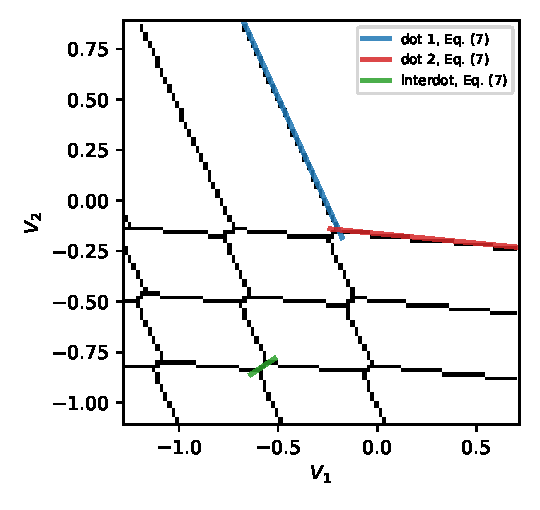
\includegraphics[width=0.46\linewidth]{figures/slopes.pdf}
\caption{Slopes predicted by Eq.~\eqref{eq:slope}, drawn over the
segments they were tested on. The interdot segment is too short to fit.}
\label{fig:slopes}
\end{figure}

\paragraph{Example: spacing.} Adding one carrier to dot~1 shifts the
constant in Eq.~\eqref{eq:degen} by $2C^{-1}_{11}$, while moving along
$V_1$ changes it at the rate $2A_{11}$. Successive dot-1 lines are
therefore $\Delta V_1 = C^{-1}_{11}/A_{11} = \dVone$ apart along $V_1$,
and dot-2 lines $\Delta V_2 = C^{-1}_{22}/A_{22} = \dVtwo$ apart along
$V_2$ --- about four and a half and three lines across the 2-unit
window, which is what Fig.~\ref{fig:states} shows.

\paragraph{The energy along a cut.} Fig.~\ref{fig:cut} follows a
straight cut through the window from lower left to upper right. The top
panel plots every configuration's energy above the ground state; a
configuration is the ground state where its curve touches zero, and each
hand-over (dotted line) is a transition. The bottom panel is the sensor
signal on the same cut (Step 6): it steps at exactly those positions.

\begin{figure}[t]
\centering
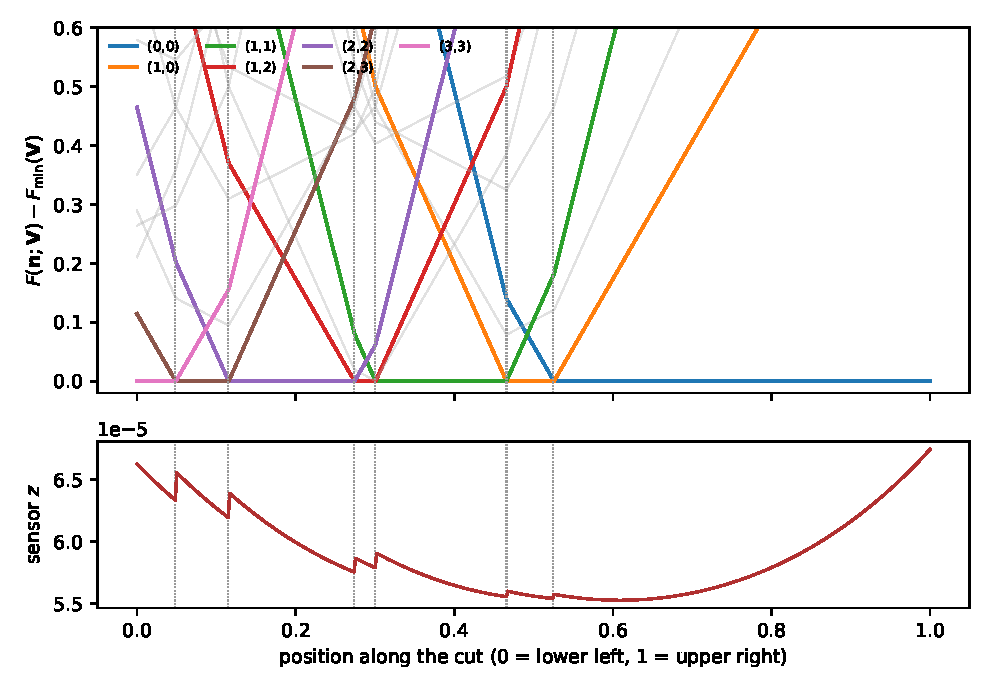
\includegraphics[width=0.86\linewidth]{figures/energy_cut.pdf}
\caption{Top: $F(\n;\V)-\min_{\n}F$ along a diagonal cut, for every
configuration within 0.6 of the ground state; the ones that become the
ground state are coloured. Bottom: sensor signal $z$, Eq.~\eqref{eq:z},
on the same cut. Dotted lines: where the ground state changes.}
\label{fig:cut}
\end{figure}

% ---------------------------------------------------------------------------
\section{Step 5 --- the label the network is trained on}

The label is computed from the ground state, not from the sensor. In
\code{dqd_simulator._charge_state_changes} a pixel $(i,j)$ is marked 1
when its occupation differs from the pixel above or to the right:
\begin{equation}
y_{ij} = \big[\,\n^*_{i+1,j}\neq\n^*_{ij}\ \ \text{or}\ \
\n^*_{i,j+1}\neq\n^*_{ij}\,\big].
\label{eq:label}
\end{equation}
This gives a $99\times99$ array, padded with a row and a column of zeros
to $\res\times\res$. Re-computing Eq.~\eqref{eq:label} from our own ground
state reproduces the stored \code{ground_truth_labels.npy} exactly. For
\devname, $\linefrac\,\%$ of the pixels are on a line (the dataset mean
quoted in the paper is 7.1\,\%).

Two consequences follow directly.
\begin{itemize}
\item The lines are one pixel wide and sit on the boundary between
states, displaced by at most one pixel from the exact degeneracy line of
Eq.~\eqref{eq:degen}: that is the pixel quantisation the tolerance
$\tau$ of the paper is designed to absorb.
\item \textbf{Interdot lines are in the label} even where the sensor
barely responds to them, because the label only asks whether $\n^*$
changed. The code comment says this is deliberate.
\end{itemize}

The label is built by a \emph{separate} QArray model,
\code{DotArray(Cdd, Cgd, charge_carrier="hole")}, which has no sensor.
The sensor map is built by \code{ChargeSensedDotArray}. The two use the
same dot-only $C$ and $\Cg$ for the ground state (the sensor enters only
the sensor signal), and for \devname\ they give the same occupation at
every pixel (Table~\ref{tab:checks}).


% ---------------------------------------------------------------------------
\section{Step 6 --- the charge-sensor signal}
\label{sec:sensor}

For the sensor, QArray adds it as a third island and repeats
Step~1 with $3\times3$ matrices. The sensor row of the non-Maxwell dot
matrix is $C_{ds}^{\rm nm}$ and its diagonal entry is \emph{zero}, so its
total capacitance is only the sum of its couplings:
\begin{equation}
C_{\rm full} = \Cfull,\qquad
C_{\rm full,\,ss} = \textstyle\sum C_{ds}^{\rm nm} + \sum C_{gs}^{\rm nm}
= \sSens .
\end{equation}
With the dots held in their ground state $\n^*$, QArray rounds the
sensor's induced charge to an integer $N_s$, evaluates the full energy
$F_k = F_{\rm full}\big((\n^*, N_s+k);\V\big)$ for
$k=-\npeak,\dots,\npeak$, and sums a Lorentzian of width $\gamma=\gam$
over the energy steps:
\begin{equation}
z(\V) = \sum_{k=-\npeak}^{\npeak-1}
\frac{1}{1+\big[(F_{k+1}-F_k)/\gamma\big]^2}.
\label{eq:z}
\end{equation}
$F_{k+1}-F_k$ is the energy to add one carrier to the sensor; a Coulomb
peak is where it vanishes. When a dot's occupation changes, the
off-diagonal terms of $C_{\rm full}^{-1}$ shift that energy, and $z$
jumps: the steps in Figs.~\ref{fig:cut} and \ref{fig:sensor}.
Eq.~\eqref{eq:z} re-implemented reproduces QArray's
\code{charge_sensor_open} at every pixel (largest difference: \zmaxdiff).

\paragraph{Where the sensor sits.} Over the window of \devname, $z$ lies
between $\zlo\times10^{-5}$ and $\zhi\times10^{-5}$ of the peak height 1,
and the smallest $|F_{k+1}-F_k|$ anywhere is $\detmin$, i.e.\
$\detminovergam\,\gamma$. The sensor is therefore never near a Coulomb
peak: it operates deep in the tail of the Lorentzian, where $z$ falls off
roughly as $\gamma^2/(F_{k+1}-F_k)^2$. An experimental sensor is usually
tuned to the flank of a peak, where the response is largest. The steps
are still exact and noise-free here, so the reconstruction task is not
affected; but it is a difference from an experiment worth knowing when
the method is transferred. This has been checked for \devname\ only.

\begin{figure}[t]
\centering
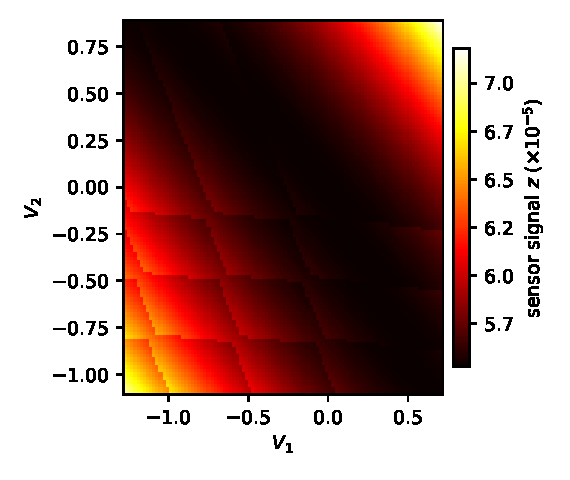
\includegraphics[width=0.5\linewidth]{figures/sensor.pdf}
\caption{Sensor signal $z$ of \devname\ from Eq.~\eqref{eq:z}; identical
to QArray's output. The smooth background is the Lorentzian tail; the
honeycomb is the steps.}
\label{fig:sensor}
\end{figure}

% ---------------------------------------------------------------------------
\section{Checks}

Every equation above was re-implemented without calling QArray's
functions and compared with QArray and with the stored files of
\devname.

\begin{table}[h]
\centering
\caption{Independent re-implementation against QArray and the stored
data, \devname.}
\label{tab:checks}
\begin{tabular}{ll}
\toprule
comparison & result\\
\midrule
\checktable
\bottomrule
\end{tabular}
\end{table}

% ---------------------------------------------------------------------------
\section{What this means for the paper}

\begin{itemize}
\item The sensor map and the label come from the same ground state, so
the lines the network is asked to draw are exactly the ones that produce
the steps in the sensor signal --- plus the interdot lines, which the
label contains even where the sensor hardly sees them.
\item Every line is straight, with a slope fixed by the lever-arm matrix
$A$; the honeycomb spacing is fixed by $C^{-1}_{ii}/A_{ii}$. Both vary
from device to device because all 14 capacitances are drawn
independently (Table~I of the paper).
\item The simulation is at zero temperature and noise-free
(\code{NoNoise}); the only broadening is the Coulomb-peak width $\gamma$
of the sensor.
\item The sensor dot has no capacitance to ground, and in \devname\ it sits
far from any Coulomb peak. Neither affects where the lines are, which is
what the study measures.
\end{itemize}

\paragraph{Reproducing this note.}
\begin{verbatim}
python docs/simulation_physics/make_note.py
cd docs/simulation_physics && latexmk -pdf simulation_physics.tex
\end{verbatim}
The script reads the device from
\code{data/_device_pools/devices_n550_res100_c1df7b6bf/sample_10}.

\end{document}
